\begin{equation}
    \begin{gathered}
        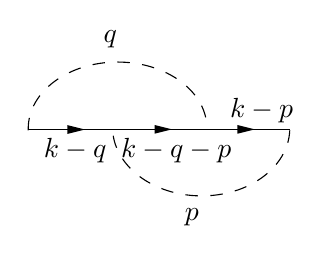
\begin{tikzpicture}[x=0.75pt,y=0.75pt,yscale=-0.7,xscale=0.7]
            %uncomment if require: \path (0,300); %set diagram left start at 0, and has height of 300
            
            %Straight Lines [id:da10067367186322329] 
            \draw    (96,175) -- (276,175) ;
            %Straight Lines [id:da263219676634183] 
            \draw    (135,175.12) ;
            \draw [shift={(135,175.12)}, rotate = 180] [fill={rgb, 255:red, 0; green, 0; blue, 0 }  ][line width=0.08]  [draw opacity=0] (12,-3) -- (0,0) -- (12,3) -- cycle    ;
            %Shape: Arc [id:dp7293618732725813] 
            \draw  [draw opacity=0][dash pattern={on 4.5pt off 4.5pt}] (96.01,175.62) .. controls (96,175.22) and (95.99,174.82) .. (95.99,174.42) .. controls (95.99,149.15) and (123.53,128.67) .. (157.5,128.67) .. controls (191.11,128.67) and (218.42,148.72) .. (218.99,173.63) -- (157.5,174.42) -- cycle ; \draw  [dash pattern={on 4.5pt off 4.5pt}] (96.01,175.62) .. controls (96,175.22) and (95.99,174.82) .. (95.99,174.42) .. controls (95.99,149.15) and (123.53,128.67) .. (157.5,128.67) .. controls (191.11,128.67) and (218.42,148.72) .. (218.99,173.63) ;
            %Shape: Arc [id:dp3248985164010143] 
            \draw  [draw opacity=0][dash pattern={on 4.5pt off 4.5pt}] (275.98,175.72) .. controls (274.91,201.11) and (247.66,221.19) .. (214.46,220.8) .. controls (181.88,220.41) and (155.49,200.45) .. (154.08,175.69) -- (215.02,173.88) -- cycle ; \draw  [dash pattern={on 4.5pt off 4.5pt}] (275.98,175.72) .. controls (274.91,201.11) and (247.66,221.19) .. (214.46,220.8) .. controls (181.88,220.41) and (155.49,200.45) .. (154.08,175.69) ;
            %Straight Lines [id:da9543303217791992] 
            \draw    (195,175) ;
            \draw [shift={(195,175)}, rotate = 180] [fill={rgb, 255:red, 0; green, 0; blue, 0 }  ][line width=0.08]  [draw opacity=0] (12,-3) -- (0,0) -- (12,3) -- cycle    ;
            %Straight Lines [id:da6776482937810475] 
            \draw    (252,175) ;
            \draw [shift={(252,175)}, rotate = 180] [fill={rgb, 255:red, 0; green, 0; blue, 0 }  ][line width=0.08]  [draw opacity=0] (12,-3) -- (0,0) -- (12,3) -- cycle    ;
            
            % Text Node
            \draw (105,179.08) node [anchor=north west][inner sep=0.75pt]    {$k-q$};
            % Text Node
            \draw (146,105.4) node [anchor=north west][inner sep=0.75pt]    {$q$};
            % Text Node
            \draw (202,227.4) node [anchor=north west][inner sep=0.75pt]    {$p$};
            % Text Node
            \draw (158.08,179.09) node [anchor=north west][inner sep=0.75pt]    {$k-q-p$};
            % Text Node
            \draw (233.08,152.09) node [anchor=north west][inner sep=0.75pt]    {$k-p$};
            \end{tikzpicture}            
    \end{gathered} \quad  \sim e^4 \int \dd[3]{\vb*{q}} \frac{1}{q^2} \int \dd[3]{\vb*{p}} \frac{1}{p^2} \sim \text{finite value},
\end{equation}